In this section we will cover the parallelization of symbolic regression and in this context detail the design choices we made in our approach.

\subsection{Approaches}
In this discussion we distinguish between fine grained parallelism and coarse grained parallelism. 

\paragraph{Fine grained parallelism}
In fine grained parallelism we parallelize a single step in the algorithm, where we execute a number of tasks in parallel that are independent of each other and where each task has a relative short completion time. 
The evaluation of the fitness function is a prime example of such a task. Evaluating fitness functions takes up the greatest part of the runtime in the algorithm.
The fitness evaluation itself can be quite complex, but in comparison with the entire runtime of the algorithm the computational cost of a single calculation is small. In order to efficiently parallelize such a taskset we have to employ a mechanism that has minimum overhead. Shared memory parallelism using threads is ideal for this use case. Optimizations such as dynamically allocated threadpools will reduce the overhead even further, and thus increase the speedup. Overhead is split over the implementation overhead of starting, assigning and administering a thread, and the copying of the problem data and its solution. Shared memory implies a near zero cost in copying, only a reference is copied. A lock on the shared data is not needed, since the instance the thread operates on is not used by any other part of the program while the fitness function is executed. This savings both code complexity and synchronization overhead.

\paragraph{Coarse grained parallelism}
In coarse grained parallelism we run a series of tasks in parallel that have a long runtime or complex workload. In our setting an example of coarse grained parallelism is running the entire algorithm in parallel, with several instances tackling a distinct subset of the problem as separate processes. Because task now has a longer runtime of the task, the overhead of parallelizing the problem can be significantly greater without impacting the speedup obtained. Typically we only start and stop such a task once, in contrast with fine grained tasks which are constantly started and then stopped again. We can use processes or threads for this form of parallelism. Threads have the benefit of being lighter in comparison to processes in terms of overhead. If we allow communication between the tasks threads can elide copying the data, at the cost of introducing locks. Processes typically have to copy data in order to communicate. We can compare both approaches with an interrupt based approach versus message passing. Whichever we choose, communication between tasks requires synchronization of some form. This introduces not only memory and time overhead, but also significantly complicates the implementation. Invariants that hold in sequential implementations are no longer guaranteed in parallel, and a careful implementation is required. 

\paragraph{Our approach}

\subparagraph{Evaluating fine grained parallelism}
Python has poor support for shared memory parallelism. While threading is available, it will not offer a speedup except for IO bound tasks due to the presence of global lock in the interpreter (GIL). It is possible to use compiled extensions in C to work around this issue, at a high cost in code complexity. A prototype implementation that parallelized the fitness function calculation proved that both threading and processes are unable to offer any speedup, often even running slower than sequential. A large part of this cost is due the overhead of copying Python objects, which are reference counted and thus require a graph traversal in order to create full copies. In order to evaluate a population of n expression trees of depth between 5 and 10 in parallel, we have to first copy the n expressions to each of the n processes, then evaluate the tree, and then copy the result back. The copying operation is orders of magnitude more expensive than the evaluation function, with both scaling exponentially with the depth of the tree. A prototype using threads elided the copy, but the GIL ensured that performance was lower than the sequential approach.
This ruled out fine grained parallelism in CSRM.

\subparagraph{Evaluating coarse grained parallelism}
We create k processes, and give each an instance of the algorithm to execute in parallel. Communication is done via message passing. We use the MPI framework, which offers Python bindings, to allow processes to communicate and synchronize. Copying is still costly, but now a speedup is possible. Threading did not work in this approach due to the GIL.
CSRM uses a set of communicating processes in order to solve the distributed SR problem.

\subsection{Distributed SR}
We will now discuss the benefits of the distributed (coarse grained) application to our problem.

\paragraph{Motivation}
A parallel metaheuristic has the obvious advantage of speedup in comparison with a sequential implementation. By dividing the problem over k processes we can, in ideal circumstances, obtain a speedup linear in k. With speedup we then refer to the time, or number of evaluations, needed to reach a certain threshold of fitness. The advantages of parallelization do not stop with this speedup. We can view the parallel processes as a swarm in itself, where each instance communicates with the others using a predefined pattern. Instead of k standalone processes we now have a set of k cooperating  processes. Each process can now use the information of others to improve its own search. Using this approach a superlinear speedup is possible. There are, however, downsides. Communication implies overhead, not only in memory but also in synchronization. Without communication the only obstacle to obtain a linear speedup is dependent on the implementation. If we compare with the sequential process we need to clearly define measures to do so. If we run k processes, each with a population p, for g generations in r phases the entire process has executed k * p * g * r iterations. We cannot find an exact equivalent in the sequential algorithm. We could run the sequential algorithm k*r phases in order to simulate the same workload but the sequential and parallel algorithms will be different search processes. Increasing the phases or generations can easily lead to overfitting. Giving a sequential algorithm a population of k*p is not equivalent to the parallel algorithm. If we increase the population we need more generations and phases. If the number of generations is less than the population size not all expressions will have been able to use combine using crossover. Finally each of the k processes starts in a different part of the search space, on a different sample of the data. There is no direct translation between k parallel processes and a sequential process. 
In this work we will focus on the improvement in the quality of solution. We will measure the difference in quality of solution between the parallel implementations and with a single sequential process. 

\paragraph{Constraints}
With communication we introduce synchronization constraints which can bottleneck a subset of the processes, or in the worst case serialize the entire group. Our aim is to to exchange the most valuable information with the least amount of overhead. This balance is problem specific, the cost of copying depends on what exactly is being copied when and to whom it is sent. Even if we restrict us to a 1-1 link between two processes, and only exchange the fittest expressions between the two processes, we do not know in advance how large the expression we copy will be, as the depth and sparseness of the tree representing the expression will vary.
While each process is given an equal sized subproblem, there are no guarantees that the actual workload of the different processes will be equal. We know that the evaluation of the fitness function has variable computational load. The stochastic nature of the metaheuristics used in the SR implementation compound this issue. By virtue of the problem statement we do not know the optimal 
solution to our problem, and with different starting points convergence between the different processes is likely to differ. We will address each of these issues.

\subsection{Topology}
A topology in this context is the set of communication links between the processes. The topology determines the convergence behavior of the entire group. In a disconnected topology, there is no diffusion of information. If a process discovers a highly fit expression, that knowledge has to be rediscovered by the other processes. The only edge case where this is an advantage is if we see the group of processes as a multiple restart versions of the sequential algorithm. If the risk for premature convergence due to local optima is high, we can try to avoid those optima by executing the algorithm in k instances, without communication. 
The implementation should offer the process an efficient way to lookup both processes from which it will receive information (sources) and processes it has to send to (targets). Source lookup is needed in order to solve the synchronization problem. Any topology that contains a cycle between processes can introduce a potential serialization effect at runtime.

\paragraph{Diffusion and concentration}
Our aim is for the processes to share information in order to accelerate the search process. With a topology we introduce two concepts : concentration and diffusion. Concentration refers to processes that share little or no information and focus on their own subset of the search space. Like exploitation concentration can lead to overfitting and premature convergence. It is warranted when the process is nearing the global optimum. Diffusion, in this work, is the process of sharing optimal solutions with other processes. Diffusion accelerates the optimization process of the entire group. It is not without risk, however. If diffusion is instant, a single suboptimal solution can dominate the other processes, leading to premature convergence. 
The topology will determine the synchronization characteristics of the processes, as well as the balance between diffusion and concentration.

\paragraph{Synchronization}
Synchronization between the processes will play an important role. While it does not directly influences convergence, it will constrain the runtime performance of the entire group. If we denote $S_i$ and $T_i$ as the set of processes that are sources and targets respectively for process i, we would like have $S_i$ minimal. The message processing code will have to wait for the slowest processes in $S_i$ before continuing. Without asynchronous communication process i would have to wait even longer, with the slowest process blocking the receipt of messages from the other processes. Synchronization implies that process i cannot send until its receiving stage has completed. If $S_i \cap T_i \neq \emptyset$ we have a cyclic dependency which can introduce deadlock in the implementation. By extension, if there is a cycle in the topology between any i, j processes this deadlock is a real risk. Dealing with this in the communication code is non trivial. We will show in section \ref{subasync} how CSRM is able to deal efficiently with cycles in the topologies that it implements. Even with deadlock resolved, cycles will introduce a tendency for the the processes to serialize on the slowest process in the node. The time spent waiting in the communication stage is lost to the convergence process. We will show how this is mitigated in our implementation.

\subsubsection{Grid}
This topology arranges a set of k processes in a square 2D grid. Each process is connected with neighbouring processes along the dimensional axes. Some variations include diagonal links, or create 3 or higher dimensional meshes. The general idea behind the grid remains invariant in those configurations. 
A grid connects all processes, allowing for diffusion of the best solution to each individual process. The key observation here is that diffusion is gradual. While a process has an immediate neighbourhood, reaching all processes takes a variable amount of communication links. Diffusion of a dominating solution will take time, and if the solution is suboptimal this time allows the other processes to evolve their own optimal solutions thereby preventing premature convergence. This risk is only mitigated by gradual diffusion, not eliminated. Elimination is only possible in the extreme case by an absence of communication or in a more advanced configuration the usage of cliques. 
Nodes on the borders of the grid communicate with their counterparts at the mirrored side of the grid. This ensures that the communication process is symmetric. CSRM supports both square grids, where k is square of natural number, or incomplete squares. 
If $\sqrt{k} \neq n $ for some $n \in \mathbb{N}$ we create a grid that would fit j processes with j given by 
\[\forall j \in \mathbb{N} \min(j) > k \land \sqrt{j} = n \] 
This grid is filled row by row with k processes. This configuration should be avoided, as the communication pattern will not always be symmetrical. It is implemented to allow a fair comparison with other topologies where the processcount is not a square. In Figure \ref{fig:topologies}\subref{subfig:grid} we see the communication pattern in a grid with 9 processes.

\paragraph{Cost}
The communication cost for k processes in a single iteration, with m messages sent per exchange, is in our configuration 4 mk.
The synchronization constraints are high, all processes are interdependent (directly or at most $\sqrt{k}$ links removed).
The lookup of targets is static, at configuration each parallel process is given a simple integer indexed mapping, the symmetry of the mapping simplifies the lookup code.

\subsubsection{Wheel}
A wheel or circle topology connects all processes with a single link shared between each source and target. Diffusion is slower than compared to the grid. For k processes it takes k-1 iterations for a message to reach all processes. Some variations introduce a 'hub', with spokes reaching out to the circle itself, completing the wheel analogy. CSRM implements this topology as a simple circle without hub or spokes. A spoked wheel topology, if the hub has bidirectional communication with all processes, has a maximum distance of 2 between all processes offering fast diffusion. Without a hub but with bidirectional links the maximum distance is $\frac{k}{2}$. A unidirectional variant is shown in Figure \ref{fig:topologies}\subref{subfig:wheel}.

\paragraph{Cost}
For k processes with m messages sent per exchange the communication cost is km. This is a static configuration with symmetric lookup. A circle is a cycle, this results in high synchronization constraints. The variant with hub and spokes introduces even higher synchronization constraints. At a doubling of message cost the doubly linked circle has an significantly higher synchronization cost than the singly linked variant. 

\subsubsection{Random}
In this topology a process selects a random target. We can configure it to do so statically, such that the target remains invariant at runtime, or select a new target after each phase. The number of targets is variable as well. CSRM implements all variants, allowing for both dynamic and static random topologies with a variable amount of targets per sending process. 
The idea behind a random topology is that it avoids communication patterns that are present in the structured topologies. If such a pattern leads to premature convergence, poor synchronization or fails to gain from the exchange of information between the processes there exists a possibility that a random approach can work. The downside is that we do not know what the maximum distance is between two processes, or even if they are connected. Cliques or cycles can form in the topology. Avoiding or detecting these requires more complex code than a simple random assignment of targets. By increasing the number of targets we decrease the probability for cliques while increasing the probability for cycles. Increasing targets will minimize the distance between two processes but increases synchronization and memory overhead.
CSRM does not enforce constraints such as clique or cycle forming in its random topologies. In Figure \ref{fig:topologies}\subref{subfig:clique} we see how a clique of cycles created by a random static configuration. A configuration with 2 links per process is shown in Figure \ref{fig:topologies}\subref{subfig:randomstatic}.

\paragraph{Cost}
The cost for a singly linked random static topology of k processes with m messages per exchange is clearly km. Synchronization constraints are unknown, and would have to be resolved by the processes. Cyclic dependencies between the processes are likely.
The lookup code for a static configuration is simple, symmetric and fast. For a dynamic configuration the lookup is simple, but only symmetric at single points in time. This observation is important because the virtual time of a process will diverge from that of the other processes. By allowing a dynamic configuration we introduce a new type of synchronization constraint. In CSRM processes have a copy of the global topology, but this is now no longer immutable. In order to resolve sources the process has to know the virtual time of the other processes. The topology remains deterministic, the seed used is identical between each process. Synchronization is highly complex in a random dynamic topology as cycles and cliques vary over time.

\subsubsection{Tree}
We introduce a binary tree topology. The links are unidirectional, with a single root and a given depth. The processcount should ideally be $k = 2^{d+1} -1$ for some $d > 0 \in \mathbb{N}$ to create full binary tree. This is not a hard constraint, for values of not satisfying the constraint we construct a tree of depth $ d =\lfloor\log_2{k}\rfloor$ and fill the last level left to right until all processes are assigned a position. Communication is unidirectional, from the root to the leaves. This topology is free from cliques or cycles. The leaves act as sinks, while the root is a source. Lookup is fast, static and symmetric. Each process except the leaves has at most two targets, and one source (except the root). The tree topology offers a structured balance between diffusion and concentration. The distance between two processes range from 1 to $\log_2{k}$. In the case of leaves the distance is infinite. Note that depending on the communication strategy, each subtree behaves as a sink. The subtrees will not share information instead concentrate on distinct parts of the search space.
A variant on this topology is a singly linked list, where the maximum distance is k. The problem with this topology is that its diffusion scales linearly with k. The full binary tree configuration is shown in Figure \ref{fig:topologies}\subref{subfig:tree}.
An alternative to this configuration is an inverted tree. If we invert all edges we now have for a tree of depth d $2^d$ leaves as independent processes feeding their best expressions to $2^{d-1}$ nodes. Instead of each process receiving at most from 1 other process their best solutions, each non leafprocesses will now receive from two other processes. Diffusion in this topology is best described in terms of shared knowledge. As we go up the tree from the leaves each node progressively learns more of this shared knowledge. In this variant a node receives knowledge from both subtrees, instead of distributing it over its subtrees.
%Link to future work.

\paragraph{Cost}
For k processes and m messages per exchange (k-1)m messages are exchanged per iteration. Synchronization overhead is minimal, there are no cycles and a process is influenced at most by $\log_2{k}$ other processes and influences at most k-1. With the exception of a disconnected topology the tree topology allows for the fastest speedup compared with grid, random and circle. 
The tree topology offers a structured alternative to the grid topology, with a staggered diffusion pattern. 
The tree topology saves a factor 4 in messaging cost compared to the grid topology. While this factor is constant, its effects are significant. 
For the same messaging cost a process in a grid topology can send trees of depth d, whereas in the tree topology it can send trees of depth d+2. This difference in depth allows for more expressive trees that can result in higher fitness value for the same communication cost. The disadvantage is that total diffusion is no longer possible.

\subsubsection{Disconnected}
The disconnected topology has zero diffusion and an infinite distance between processes. The only applications of this topology are in cases where the risk for premature convergence due to diffusion is high and can for some reason not be mitigated. Secondly it can serve as a comparison with the other topologies in order to measure the diffusion effect, memory and synchronization cost. 

\paragraph{Cost}
Cost is near zero, no messages are sent nor is any synchronization needed. In practice the collecting of all results will still have to be done by either an elected process or a process statically assigned as collector. This holds true for all topologies.

\subsection{Asynchronous communication}\label{subasync}
We have to tackle deadlock and synchronization delay in our parallel implementation. We will first describe the interaction between the processes and using this context demonstrate our solution.

\paragraph{Control flow}
The control flow of our parallel SR process is shown in Figure \ref{fig:parallelflow}.
A parallel process in our implementation executes a single phase of the algorithm, then collects at most m of its fittest expressions from the archive. 
The set of target processes is resolved using the topology, then the m messages are send to the targets. 
After the sending stage the process looks up its sources using the topology, and waits for messages from those sources. 
The received messages are decoded to expressions which are used by the algorithm for its next phase. The algorithm stores the expressions in its archive and then uses that archive to reseed the next phase. The archive is used for both external input and the best solutions from the previous phases. Since the archive has a fixed size, it will introduce an evolutionary pressure. A new expression will replace an existing if its fitness value is strictly lower. Allowing expressions with equal fitness values to replace each other can be useful in some cases where it allows the optimization process to traverse zero gradient areas in the topology of the fitness function. It can also lead premature convergence where a large subset of the fittest population holds identical fitness values with low to no diversity. CSRM enforces a strict order in its population in order to prevent this last scenario. 

\begin{figure}
\begin{tikzpicture}[node distance=1.5cm, every node/.style={font=\footnotesize}]
\node (start) [startstop] {Start};
\node (phase) [decision, below of=start, yshift=-0.5cm] {Phase $<$ Phases};
\node (execute) [process, below of=phase, yshift=-1cm] {0. Execute phase};
\node (collect) [process, below of=execute] {1. Collect m best expressions};
\node (lookup) [process, below of=collect] {2. Lookup targetset T};
\node (spread) [process, below of=lookup] {3. Distribute m over T using policy};
\node (check) [process, below of=spread] {4.0 Wait until all messages from previous phase have been received by target};
\node (send) [process, below of=check] {4.1 Send m to t $\in$ T asynchronously};
\node (lookups) [process, below of=send ] {5 Lookup sourceset S};
\node (receive) [process, below of=lookups ] {6 Receive messages from s $\in$ S};
\node (seed) [process, below of=receive ] {7 Reseed algorithm using received messages};

\draw [arrow] (start) -- (phase);
\draw [arrow] (phase) -- (execute);
\draw [arrow] (execute) -- (collect);
\draw [arrow] (collect) -- (lookup);
\draw [arrow] (lookup) -- (spread);
\draw [arrow] (spread) -- (check);
\draw [arrow] (check) -- (send);
\draw [arrow] (send) -- (lookups);
\draw [arrow] (lookups) -- (receive);
\draw [arrow] (receive) -- (seed);
\draw [arrow] (seed)-- +(2,0) |- (phase) node[near start,sloped,above] {};
\end{tikzpicture}
\caption{Parallel control flow.}
\label{fig:parallelflow}
\end{figure}

\paragraph{Waiting for messages}
If a process does not wait for messages from other processes the convergence behavior of the entire group non deterministic. In most platforms there are no hard guarantees about inter process scheduling. We can end up in extreme cases with a single process only sending and never consuming messages. This would break the intent of a structured topology. While this is an extreme example, even in average cases an extra level of non determinism is introduced without there being an explicit need for it. Not waiting for messages requires that messages are buffered by the parallel framework, and this can lead to internal buffers varying in size.  We will show another approach where the deterministic execution of the parallel metaheuristic is retained. This does not imply that the process itself is no longer stochastic, only that we are guaranteed that our designed communication pattern is strictly adhered to. Our algorithm can be provided with seeds making it deterministic. Each different seed is likely to lead to a different solution, or at least a different starting point. Without determinism it becomes very difficult to accurately compare configurations of the algorithm.

\paragraph{Deadlock}
From our previous discussion we know that deadlock is a risk if there are cycles in the topology. Since each process has full knowledge of the topology (except in a random dynamic topology) it is possible to implement an algorithm that resolves deadlock by ordering the sending an receiving of the messages. Suppose A waits for B, and B for A in the most simple example. A simple solution of A sending to B, B receiving from A, then B sending to A and A receiving from B would break the deadlock. This simple interleaving solution is not unique, but the priority is not important here. As long as the deadlock is broken the processes can continue. There are 2 serious issues with this approach. First, this approach serializes concurrent processes. This is detrimental to any speedup we were hoping to achieve. Second, the implementation becomes more complex. The order of calls is no longer statically defined, we need an algorithm that acts as a central coordinator between any group of processes in a cycle, computes a solution, and executes that solution in order. We cannot directly invoke operations on other processes, so the only solution is to execute the coordinating algorithm in parallel on all processes if they detect that they are a member of a cycle. Each process will then know when it can send and receive based on the computed order. While this solves deadlock, we still end up with a serialized execution and the communication code becomes far more complex than a simple sequential sending and receiving call.

\subparagraph{Asynchronous solution}
CSRM instead opts for an asynchronous sending of messages in order to resolve deadlock and mitigate the serialization. Cycle detection is no longer needed. 
A process executes a phase, then looks up its targets for messages. Instead of sending the messages with a blocking call to the framework, the sending process now allocates a buffer and sends each set of messages to its target with an asynchronous call. It stores a future object that can later be checked to verify if the receiving process has executed its receive call. 
The order of sending is no longer relevant, the sending call returns immediately for each target. 
Next the process calls receive for each of its sources. This is a blocking call, but this does not introduce a risk for deadlock.
In the worst case our process waits until the source has stopped its own sending call, but due to its asynchronous nature this process is quite fast. The order of sources is no longer a risk for deadlock. After receiving all messages the process continues its execution as before.
Each process still has clear the allocated buffers and callback objects from its send operation. The buffers cannot be deallocated as long as the receiving process has not acknowledged receipt of the contents. In order to check this we invoke the future objects, but care must be taken here. Calling the futures for each receiving process results in a blocking call. If we time this operation incorrectly we simply have deadlock all over again. The latest a process can wait is that point in time where the send buffers are needed again, which is in the next iteration. As soon as a process enter the sending phase, the first operation it executes is waiting on the future objects. After each returning call the corresponding buffer is cleared for reuse. 
It should be clear that this approach does not simply delays deadlock but prevents it from occurring. The asynchronous approach allows the processes to interleave in any order that resolves the deadlock. Instead of an explicit algorithm, we simply let each cycle of processes resolve the deadlock in their own optimal sequence. Finally note that the receive call returns immediately once the framework has registered the corresponding send call, it is not directly waiting on the sending process.

\paragraph{Synchronization delay}
We know from our previous discussion that the execution time of a single phase will vary per process, and even between phases for a single process. The receiving of messages is a synchronization point between processes, but not a strict one as the sending process will only wait for receipt in the next phase. This means that a process will only be waiting on any other process after completion of a phase. If we introduce drift as the virtual time difference between processes, in order for processes to delay each other the drift would have to be greater than the execution time of a single phase. A strict serialization effect is therefore not possible. What we introduce with this implementation is latency buffer equal to the runtime of the next phase. The time to execute a phase, while variable, will still be on average far greater than the time needed to communicate results. One of our aims in distributing SR is obtaining a speedup by, amongst other things, finding a balance between phase runtime and communication time.

\subparagraph{Delay tolerance without cycles}
In Figure \ref{fig:delaynoncyclic} we visualize how our approach allows a faster process to avoid waiting on a slower process. Solid vertical lines are blocking calls, the line represents the time spent waiting. The receive and check calls are blocking but return immediately. The send call is asynchronous and returns immediately. Asynchronous calls start the lifetime of a future object visualized with a vertical dotted line. The object's lifetime ends with a corresponding call from another process.
The length of a phase is the delay tolerance that prevents strict serialization. We see three processes in a topology without cycles, where the phase time $t_p$ follows this pattern : $t_{pa} < t_{pb} < t_{pc}$. Process A can at most tolerate a delay of a single phase. If there is a strict ordering in average phase time between processes, then the processes will end up being serialized if the delay has exceeded a single phase. The average phase runtime will vary over time for a single process due to the ever evolving populations of differing depth and evaluation functions of varying complexity. The very fact that the runtime varies ensures that, with the exception of edge cases, the phase runtime average between processes will tend to the same values. Our approach allows the avoidance of serialization in the general case, given that the variation between the runtime will not be too extreme. The runtime of a single phase is dimensioned by the population and the number of generations. If we increase either one the runtime will increase, but the effect on the variation is far less predictable. In practice the runtime will depend on the average depth in the population, and the average complexity of the population. With the depth limited the complexity is limited as well. The only remaining variable influencing runtime is then the scheduling algorithm of the operating system. With the exception of real time operating systems there is no upper limit here, but in practice the average runtime of a process on a system that is not overloaded will tend to a constant. This means that we can estimate a distribution of the phase runtime for a single sequential process, and use the mean and standard deviation of that distribution to find a value that prevents with a high probability serialization. 
\begin{figure}
    \centering
    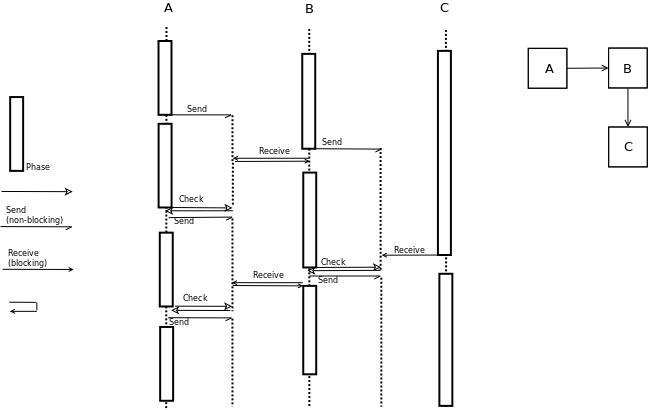
\includegraphics[width=\textwidth,height=\textheight,keepaspectratio]{figures/delay.png}
    \caption{Synchronization delay tolerance in CSRM.}
    \label{fig:delaynoncyclic}
\end{figure}

\subparagraph{Delay tolerance in the presence of cycles}
When two processes have a cyclic dependency, that is that they wait on each other's communication, the delay tolerance cannot avoid serialization. In Figure \ref{fig:delaycyclic} we see how processes A and B are serialized due to their interdependency. This cannot be avoided, process A needs the messages from B and vice versa in order to proceed. In the figure we see clearly the receive call waiting until a corresponding send call has been issues. While the send call returns immediately, the receive call has to block until send has been invoked. The same applies for the check call, until receive returns the check call blocks. In the figure the time spent waiting is visualized with a solid vertical line. 
This figure demonstrates our deadlock resolution method. If the send call would block for either process, then both A and B would wait indefinitely. By making this operation return immediately the deadlock is resolved. This generalizes to larger cycles, for example in the wheel or grid topologies. Without this implementation only tree topology or random topology with cycle detection could work.
\begin{figure}
    \centering
    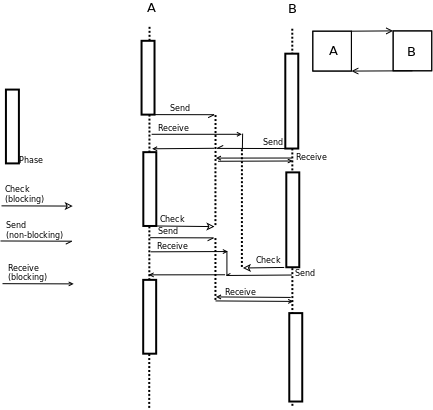
\includegraphics[width=\textwidth,height=\textheight,keepaspectratio]{figures/delaycycle.png}
    \caption{Synchronization delay tolerance in CSRM in the presence of cycles.}
    \label{fig:delaycyclic}
\end{figure}

\paragraph{Future improvements}
If we allocate a buffer per communication phase, we can wait even longer before invoking future objects. This means we can leave a configurable amount of phases before we wait on the receipt of messages. The downside of this approach is that the memory constraints for each process now signficantly increase from m to pm where p is the number of phases we opt to wait.
The receive call is executed in sequence for the list of sources in the target process. In order to minimize delay even further we could execute this call asynchronously as well. Extra code would need to be introduced to handle the non deterministic behavior this introduces. The order in which the messages are received can influence the algorithm. When the archive is seeded with these external expressions we drop any expressions with identical fitness values. There is thus a risk that by varying the order we introduce non determinism in our results. This can be resolved in the receiving code by preallocating the buffer for all sources and after all asynchronous receive calls storing the messages in the same order of the sources list. 
Asynchronous receiving is not implemented in CSRM.

\subsection{Communication strategies}
If the process has j targets, and the algorithm is configured to distribute the m best solutions, we can use several approaches to send those to their targets. We can spread m over j, using a random, interleaving, slicing or any other type of sampling technique. An alternative is copying m j times so that each target receives m messages.
CSRM has a Spreadpolicy interface that hides the implementation of this behavior for the processes. CSRM defaults to a slicing policy. If we have m messages to distribute over j targets, we will sequentially assign each of the j process $ \lfloor{m/j}\rfloor $ messages.
This policy is efficient as it avoids copying but has a direct effect on the diffusion between the processes. First of all the value of m should be chosen with the topology in mind. If m = 2 in a grid topology, each process will only send and receive 2 messages, not 4. This will alter the diffusion pattern. For a tree topology m should be 2 as well, else we create a symmetric series of cliques, which is unlikely be intended. If we use a copy policy the value of m can be as low as 1. For random topologies m depends on the parameter determining the number of targets. In our circle topology m = 1 is sufficient for both policies.

\begin{figure}
    \centering
    \begin{subfigure}{0.5\textwidth}\label{subfig:grid}
	    \centering
        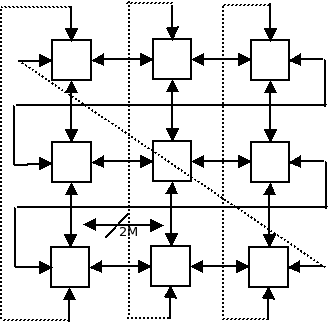
\includegraphics[width=0.6\linewidth]{figures/grid.png}
        \caption{Grid topology with k = 9.}
    \end{subfigure}
    \begin{subfigure}{0.5\textwidth}\label{subfig:wheel}
	    \centering
        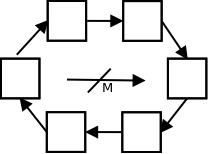
\includegraphics[width=0.6\linewidth]{figures/wheel.png}
        \caption{Circle topology with k = 6.}
    \end{subfigure}
    \begin{subfigure}{0.5\textwidth}\label{subfig:tree}
    \centering
        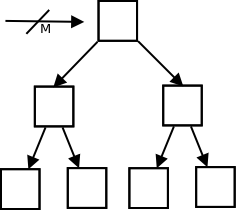
\includegraphics[width=0.6\linewidth]{figures/tree.png}
        \caption{Tree topology with k = 7}
    \end{subfigure}%
    \begin{subfigure}{0.5\textwidth}\label{subfig:randomstatic}
	    \centering
		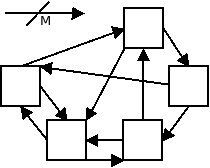
\includegraphics[width=0.6\linewidth]{figures/random.png}
		\caption{Random topology with 2 outgoing links per process, k = 5.}
    \end{subfigure}
	\begin{subfigure}{0.5\textwidth}\label{subfig:clique}
    		\centering
        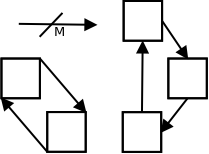
\includegraphics[width=0.6\linewidth]{figures/clique.png}
        \caption{Random topology resulting in cliques of cycles, k = 5.}
    \end{subfigure}%
    \caption{Selection of visualizations generated by CSRM.}
    \label{fig:topologies}
\end{figure}

\subsection{Exploiting parallelism for validation}

\subsubsection{Predictive capability}
In SR we try to find an expression that, based on some distance function, fits input data as close as possible to expected data. If we do not use test data to score the resulting expression, the result of overfitting is very real. Not only is it possible that the expression fits the new data points from the test set poorly, the new datapoints may fall outside the domain of the generated expression. By scoring the expression on unknown data we measure its predictive capability $P_{sr}$. In sequential mode, CSRM evolves an expression on training data, then scores the expression on the full data. We record the correlation between the fitness on the training data and the fitness on the full data in order to measure, over generations and phases, the convergence process. We would like to have an answer to the question : How does $P_{sr}$ of the SR process evolve over time?\\
This question is vital to a practitioner. If we have an indication that prediction is no longer increasing, or even decreasing we should halt the process. On the other hand if we see that a linear increase is still present we can opt for extending the runtime of the algorithm. Conventional validation, as described here, can be replaced with cross validation in order to obtain a more accurate measure for $P_{sr}$.

\paragraph{Cross validation}
Several approaches in cross validation exist. We distinguish between exhaustive and non-exhaustive methods. The first uses all possible combinations of training and test data to obtain the maximum amount of information of $P_{sr}$. Its disadvantage is a high computational cost, although this can still be linear in the length of the dataset if we omit only  a single datapoint per selection from the dataset. We will focus on k-fold cross validation (KCV), a non exhaustive validation technique. 
In KCV we split the data over k samples, then use k-1 of those as the training data and one as the validation data. The process is repeated k times, to obtain full coverage. Even though this approach is non-exhaustive it would still require k iterations of the entire algorithm.

\subsubsection{Parallelization}

\paragraph{Approximating k fold cross validation}
With the distributed implementation of SR we can avoid the factor k increase required for KCV. CSRM can, as we have shown, run n instances of the algorithm in parallel. Those instances can cooperate by exchanging their current best solutions, possibly accelerating the convergence of the entire process. Instead of translating our sequential approach to the distributed approach and giving each process the same training data, we can approximate KCV without the linear increase in runtime. We do not implement full KCV, but mimic the process. For a dataset of length d, k fold will split it into k equal sized sections of size s = $\frac{d}{k}$. Each training set has $s*(k-2)$ overlapping datapoints. The value of k determines the effect of the outcome to a large extent. We would like to keep the overlap above a certain treshold, insensitive to k. If the overlap is too small the probability of highly fit expressions proving to be invalid on the validation data becomes too large. 

\begin{figure}
    \centering
    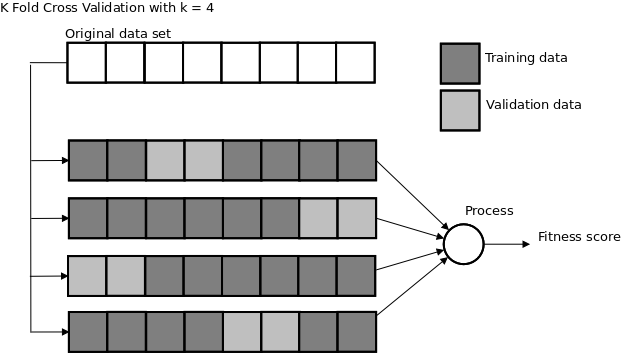
\includegraphics[width=\textwidth,height=\textheight,keepaspectratio]{figures/kfold.png}
    \caption{Visualization of k fold cross validation with k = 4.}
    \label{fig:kfold}
\end{figure}

\paragraph{Approach}
With k processes running in parallel, and d datapoints, we give each process a random sample of size r*d with $r \in [0,1]$. In practice we use r = $\frac{4}{5}$. This is the same approach we use in our sequential implementation. The difference now is that each process is given a different trainingset of size r*d, with a stochastically determined overlap threshold. Each process uses its own distinct trainingset to evolve expressions from and at the end of execution scores its population on the full data set. Each process uses a different seed for its random number generators, so we have k processes working on a different area of the search space, but there is enough shared information to make the results of each individual process relevant to each other. Our approach is visualized in Figure \ref{fig:csrmkfold} with $r = \frac{3}{4}$ and k = 4.
The probability that any two trainingsets share a single datapoint is $r^2$. This probability is invariant to k, the number of processes. So for any two communicating processes, regardless of the topology or validation process, the ratio of shared data points is constant. When two processes exchange their best expression, the new expression is scored using the receiving process' training data set. The invalid expression problem is not only present at the end of the algorithm, it is also a vital factor during the communication between the processes. If process A evolves an expression that has a high probability of being invalid on process B's trainingset, the possible gain we have in sharing that expression evaporates. By establishing a constant threshold we can mitigate this risk and still gain from the validation process.
The choice of concurrent processes is constrained in practice, typically it is determined by the available hardware or the topology. Our validation approach is insensitive to this value. 

\begin{figure}
    \centering
    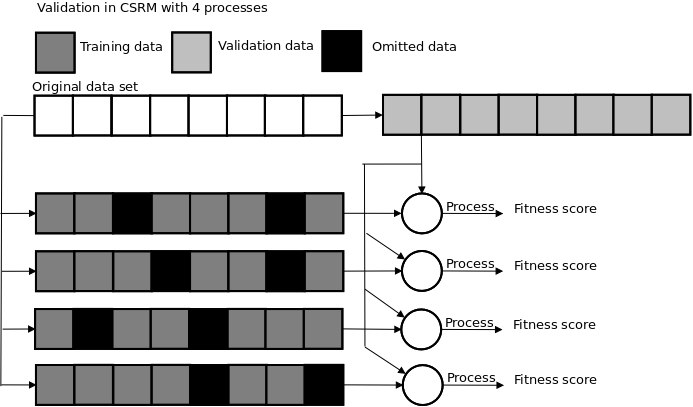
\includegraphics[width=\textwidth,height=\textheight,keepaspectratio]{figures/validationcsrm.png}
    \caption{Approximation of k fold cross validation with parallel processes, k = 4,  r = $\frac{3}{4}$.}
    \label{fig:csrmkfold}
\end{figure}

\subsection{Conclusion}
We have covered our distributed design and highlighted the issues that drove our choices. CSRM offers the practitioner several topologies each with its strengths and weaknesses. 
With a wealth of topologies and configurations we also increase the dimensions of the parameter optimization problem. In the experiments we will evaluate some, but not all parameter choices. 
Our implementation can easily be extended with more topologies or policies without risking deadlock or serialization.
Our validation approach in parallel CSRM allows an approximation of KCV without increasing the runtime cost by a factor k. The validation is insensitive to the number of processes and finds a balance between generating predictive expressions while minimizing the occurrence of invalid expressions.